\documentclass[12pt,french]{book}

\input preambule_2014
\input{perso_cecile_2014}

%réglages marges
\geometry{includeheadfoot,top=0.5cm,bottom=0.8cm,right=1.5cm,left=1.5cm}
\pagestyle{fancy}
\fancyhf{}

\fancypagestyle{garde}{% 
\fancyhead[C]{\small\textbf{Nom,  Prénom :} \makebox[5cm]{\dotfill}\hfill \small \textbf{1ES$_1$} - 2014-2015}
\renewcommand{\headrulewidth}{0cm}}




\begin{document}
\thispagestyle{garde}

\medskip

%cadre titre
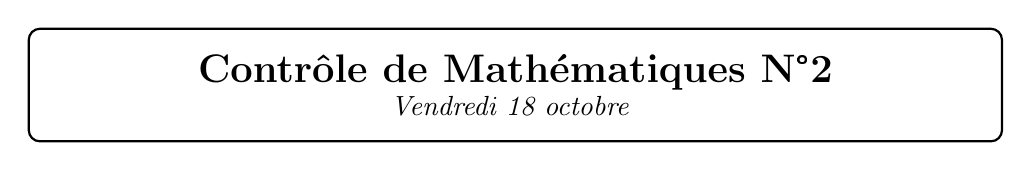
\begin{tikzpicture}
\node[rectangle,draw=black,rounded corners,thick,fill=white]{%
\begin{minipage}{\linewidth}
\begin{center}
\vspace*{6pt}
\textbf{\Large \bsc{Contrôle de Mathématiques} N°2}\par
\textit{Vendredi 18 octobre}
\vspace*{6pt}
\end{center}
\end{minipage}
};\end{tikzpicture}





% consignes

\begin{center}
\begin{minipage}{0.8\linewidth}
\begin{center}
\itshape
\textbf{Les calculatrices ne sont pas autorisées}.\par
La qualité de la rédaction, la clarté et la précision des raisonnements seront pris en compte dans l'appréciation de la copie.
Le barème est indicatif.
\end{center}
\end{minipage}
\end{center}

\noindent


%$$$$$$$$ le contrôle !$$$$$$$$$$$$$$$$$$$


\end{document}
